\documentclass[12pt, a4paper, hidelinks]{article}

% Packages:
\usepackage{graphicx}                   % For figure includes
\usepackage[T1]{fontenc}                % For mixing up \textsc{} with \textbf{}
\usepackage[utf8]{inputenc}             % For scandinavian input characters(æøå)
\usepackage{amsfonts, amsmath, amssymb} % For common mathsymbols and fonts
\usepackage[english]{babel}              % For danish titles
\usepackage{hyperref}                   % For making links and refrences
\usepackage{url}                        % Just because {~_^}
\usepackage{array}                      % ...
\usepackage[usenames, dvipsnames, svgnames, table]{xcolor}
\usepackage{tabularx, colortbl}
\usepackage{verbatim} % For entering code snippets.
\usepackage{fancyvrb} % A "fancy" verbatim (for pseudo code).
\usepackage{listings} % For boxed codesnippets, and file includes. (begin)
\usepackage{lipsum}   % For generating dummy text at this demonstration
\usepackage{enumitem}
\usepackage[section]{placeins} % prevents figures from floating
\usepackage[final]{pdfpages}   % for including the frontpage
\usepackage{makecell}          % for heavier \hlines
\usepackage{caption}           % for costum captions
\usepackage{cleveref}          % for cref

% Basic layout:
\setlength{\textwidth}{165mm}
\setlength{\textheight}{240mm}
\setlength{\parindent}{0mm}
\setlength{\parskip}{\parsep}
\setlength{\headheight}{0mm}
\setlength{\headsep}{0mm}
\setlength{\hoffset}{-2.5mm}
\setlength{\voffset}{0mm}
\setlength{\footskip}{15mm}
\setlength{\oddsidemargin}{0mm}
\setlength{\topmargin}{0mm}
\setlength{\evensidemargin}{0mm}

\newcolumntype{C}[1]{>{\centering\arraybackslash}p{#1}}

% Colors:
\definecolor{KU-red}{RGB}{144, 26, 30}

% Text Coloring:
\newcommand{\green}[1]{\textbf{\color{green}{#1}}}
\newcommand{\blue} [1]{\textbf{\color{blue} {#1}}}
\newcommand{\red}  [1]{\textbf{\color{red}  {#1}}}
% Create a figure with \fig{filename}{figure_text}
\newcommand{\fig}[3]{
\begin{figure}[h]
  \begin{center}
    \includegraphics[width=#2mm]{./img/#1}
  \end{center}
  \caption{#3}
  \label{fig:#1}
\end{figure}
}
\def\fatline{\Xhline{2\arrayrulewidth}}
\renewcommand{\arraystretch}{1.3}
\renewcommand{\tt}[1]{\texttt{#1}}
\renewcommand{\bf}[1]{\textbf{#1}}
\renewcommand{\it}[1]{\textit{#1}}

% **************** Start Document *****************
\begin{document}
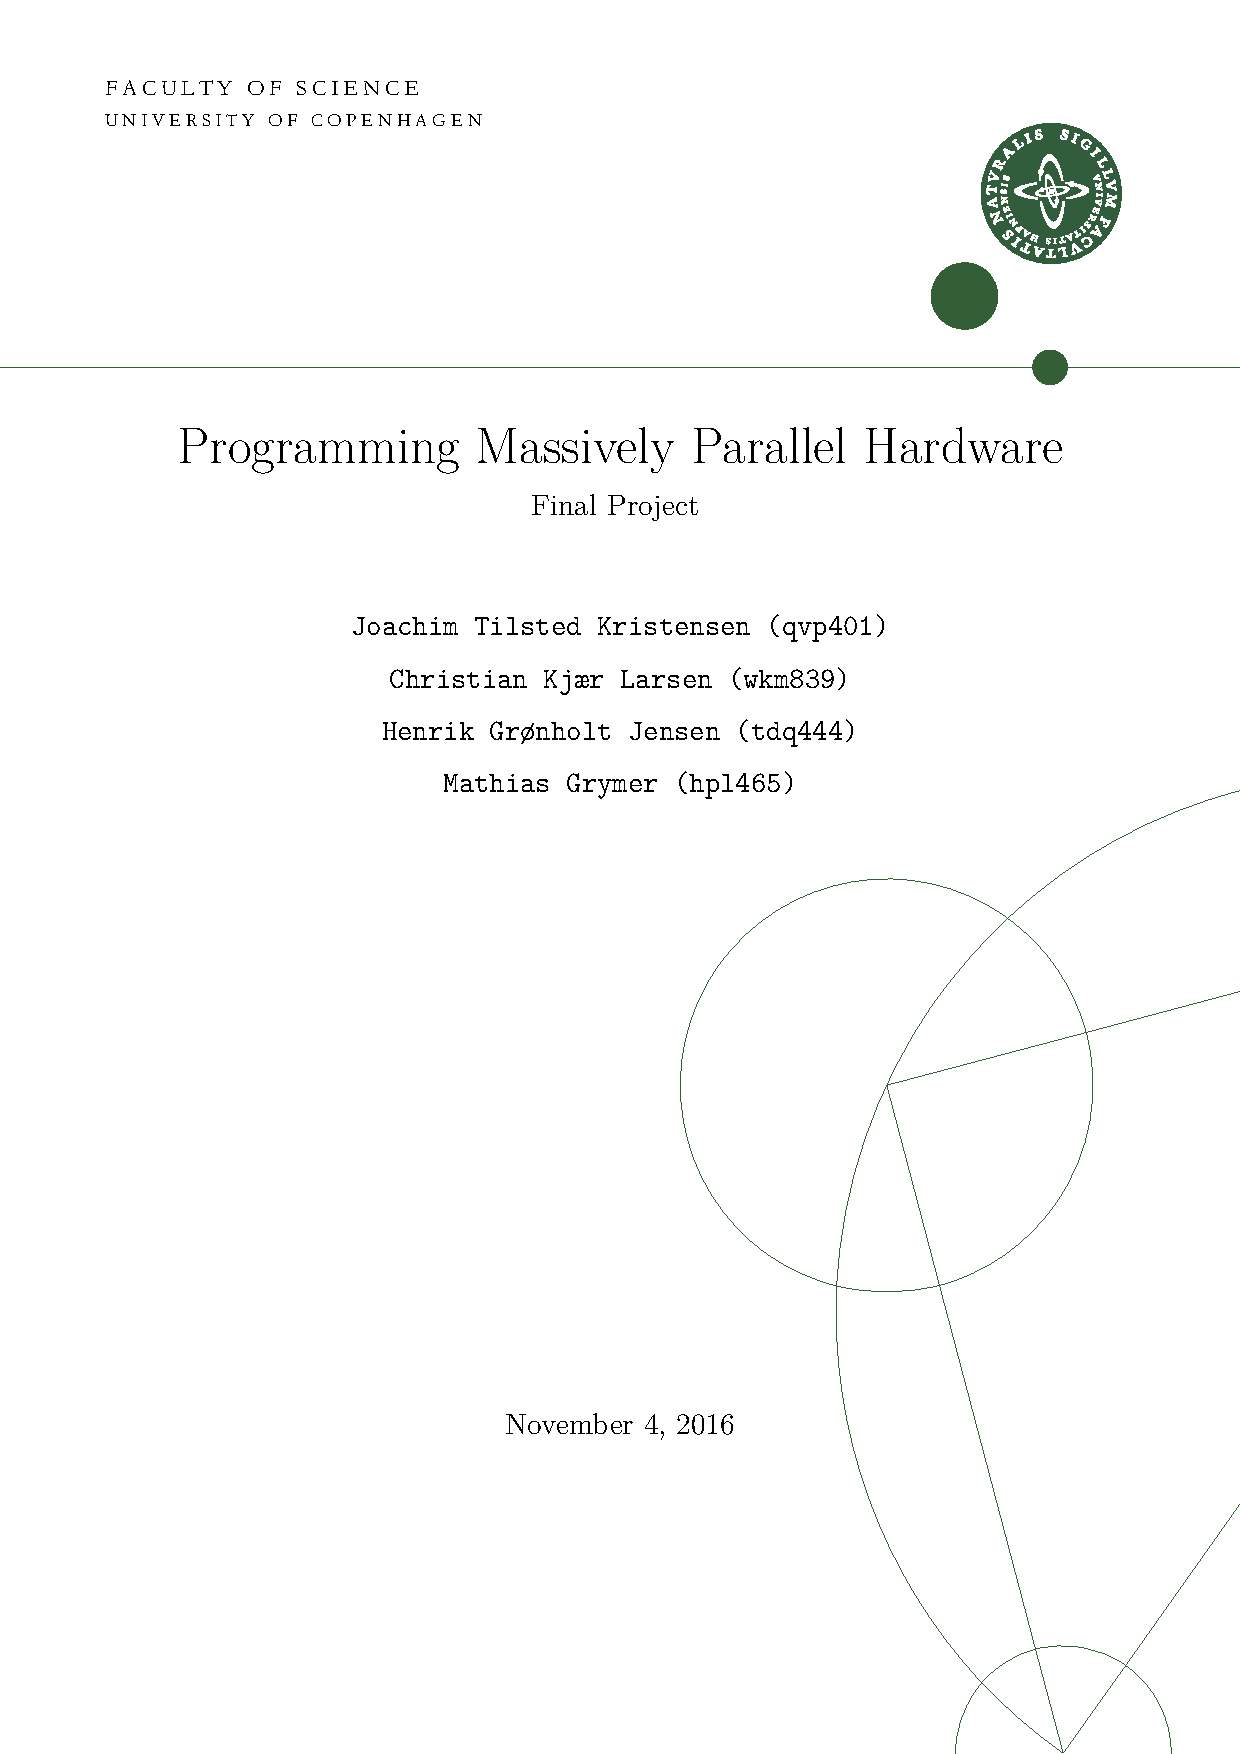
\includepdf[pages=1]{./frontpage/frontpage.pdf}
\tableofcontents
\newpage

\section{Project Introduction}
A histogram is a density estimate over a distribution of data.
It is quintessential to quality control, distribution estimation
and similarity measures when working with large datasets.
As it scales with the size of the input,
a parallel solution is preferable when the input is large.
However, when it comes to real world unsorted data,
histograms are computationally inefficient
due to the random memory access caused by
the counting of how many values fall into each bin.
In this project, we implement a CUDA-based solution for building a 1D histogram
in parallel and benchmark the scalability of our solution with
the CPU and the naive GPU versions.
We also investigate how to efficiently solve the problem when the dataset
is larger than the available (device) memory on the GPU
using streaming techniques.

\section{Design Overview - From CPU to GPU}
Building a histogram in parallel is a straightforward map-reduce problem.
It can be thought of as simplistic kernel density estimation
where a function $f$ maps frequencies of data \tt{vals} over bins \tt{inds}
and reduces by counting how many values falls into each bin.
The unoptimised pseudo-code for a 1D histogram
would look something like:

\begin{verbatim}
forall (i = 0; i < size(data); i++)
    idx = f(data[i])
    hist[idx]++ // Must be atomic
\end{verbatim}

For an efficient parallel implementation on the GPU,
the reduce-phase becomes the tricky part.
The unknown order of indices from the map-phase
prevents us from working with the data in a coalesced manner during the reduce-phase.
Our solution to this problem is to partially sort the output indices from
the map-phase into \it{segments} that are guaranteed to fit in the
shared memory of a CUDA block (i.e. no indices fall outside the subset of bins
we can hold in shared memory).\\
Each block will use its shared memory to create a local histogram
and atomically add this to a global histogram residing on the GPU.
However, to fully utilize hardware parallelism we are likely to have
each CUDA block working on a large subset of data that will
span more than one \it{segment} (local histogram).\\
The subset of data (or indices) a block handles is defined as the workload per thread
(\tt{chunk\_size}) times the number of threads in a block (\tt{\#thread\_pr\_block}).
This workload depends on the size of the input data vs.
total number of threads available, and is independent of the sorted segments.
Thus, in each block we need to know when to flush a local histogram to global
memory and start a new segment.
The problem is illustrated in \Cref{fig:overview} where e.g.
$block_0$ spans $segment_0$ and $segment_1$.

\fig{overview}{140}{General idea of the algorithm}

Letting a block handle overlapping segments (i.e. creating more local histograms)
is preferable to a more naïve implementation where a block is spawned
for each segment. This is to keep the algorithm work efficient.
The problem with a more naïve version is that there is no way
to guarantee that all blocks have roughly the same workload.
One could easily have a case where certain segments have significantly
more elements than others, leading to bottlenecks where other blocks will
wait for the overworked blocks to finish.

\section{Overview of Implementation}
In this section, we give a quick overview of our implementation. We describe
an implementation with shared memory, but without the bookkeeping needed for
histograms larger than what fits in shared memory on the GPU. Then we describe
an implementation with the proper bookkeeping for histograms of arbitrary size.
\fig{device-dia}{140}{Flow of data in our GPU implementation}

\subsection{Optimised for small histograms}
The first step towards the algorithm described previously is an implementation
for histograms less than the size of the shared memory for each CUDA block.
In our case that is 4096/8192 elements (depending on the configuration). This
is because each CUDA block has around 8000 words of memory available. The reason
for making the amount of shared memory less than this, is that the hardware can
reconfigure parts of shared memory to function as a cache, and therefore speeding
up other memory accesses.

The algorithm is roughly as follows.

\begin{itemize}
\item Reset the shared memory for the block.
\item Write the indices (\tt{f(data[i])}) into the shared memory of the block.
\item Commit the block level histogram to global memory.
\end{itemize}

\subsection{Optimised for large histograms}
To make an implementation for larger histograms, we need to do a lot more
bookkeeping. This is done in the following manner.

\begin{itemize}
\item
  Map f onto the data array
\item
  Partially sort the resulting indices into a number of equivalence classes (\it{segments})
\item
  Calculate the offset for each segment into
  the partially sorted array of indices.
  This is needed to find the segment for each block.
\item
  Reset the shared memory for each block
\item
  Write the indices into the shared memory of the block modulo the shared memory size
\item
  If we change segment,
  we commit the block level histogram to global memory with a certain
  offset and continue with the next segment in the same manner.
\end{itemize}

A flow of the code is shown on figure~\ref{fig:device-dia}.

A lot of details are left out, but they are very specific to the hardware,
and it is a lot easier just to read the CUDA implementation.
This is especially for details regarding the bookkeeping and calculation
of segment offsets.

\section{Benchmarks}
To evaluate our solution, we have benchmarked our implementation with
a sufficiently large dataset, in this case 10 million elements.
We have kept the size of the input data constant,
because we are testing whether our implementation is more
efficient when the number of bins in the histogram increases. The result
can be seen on figure~\ref{fig:graph1}.
\begin{figure}[htpb]
    \centering
    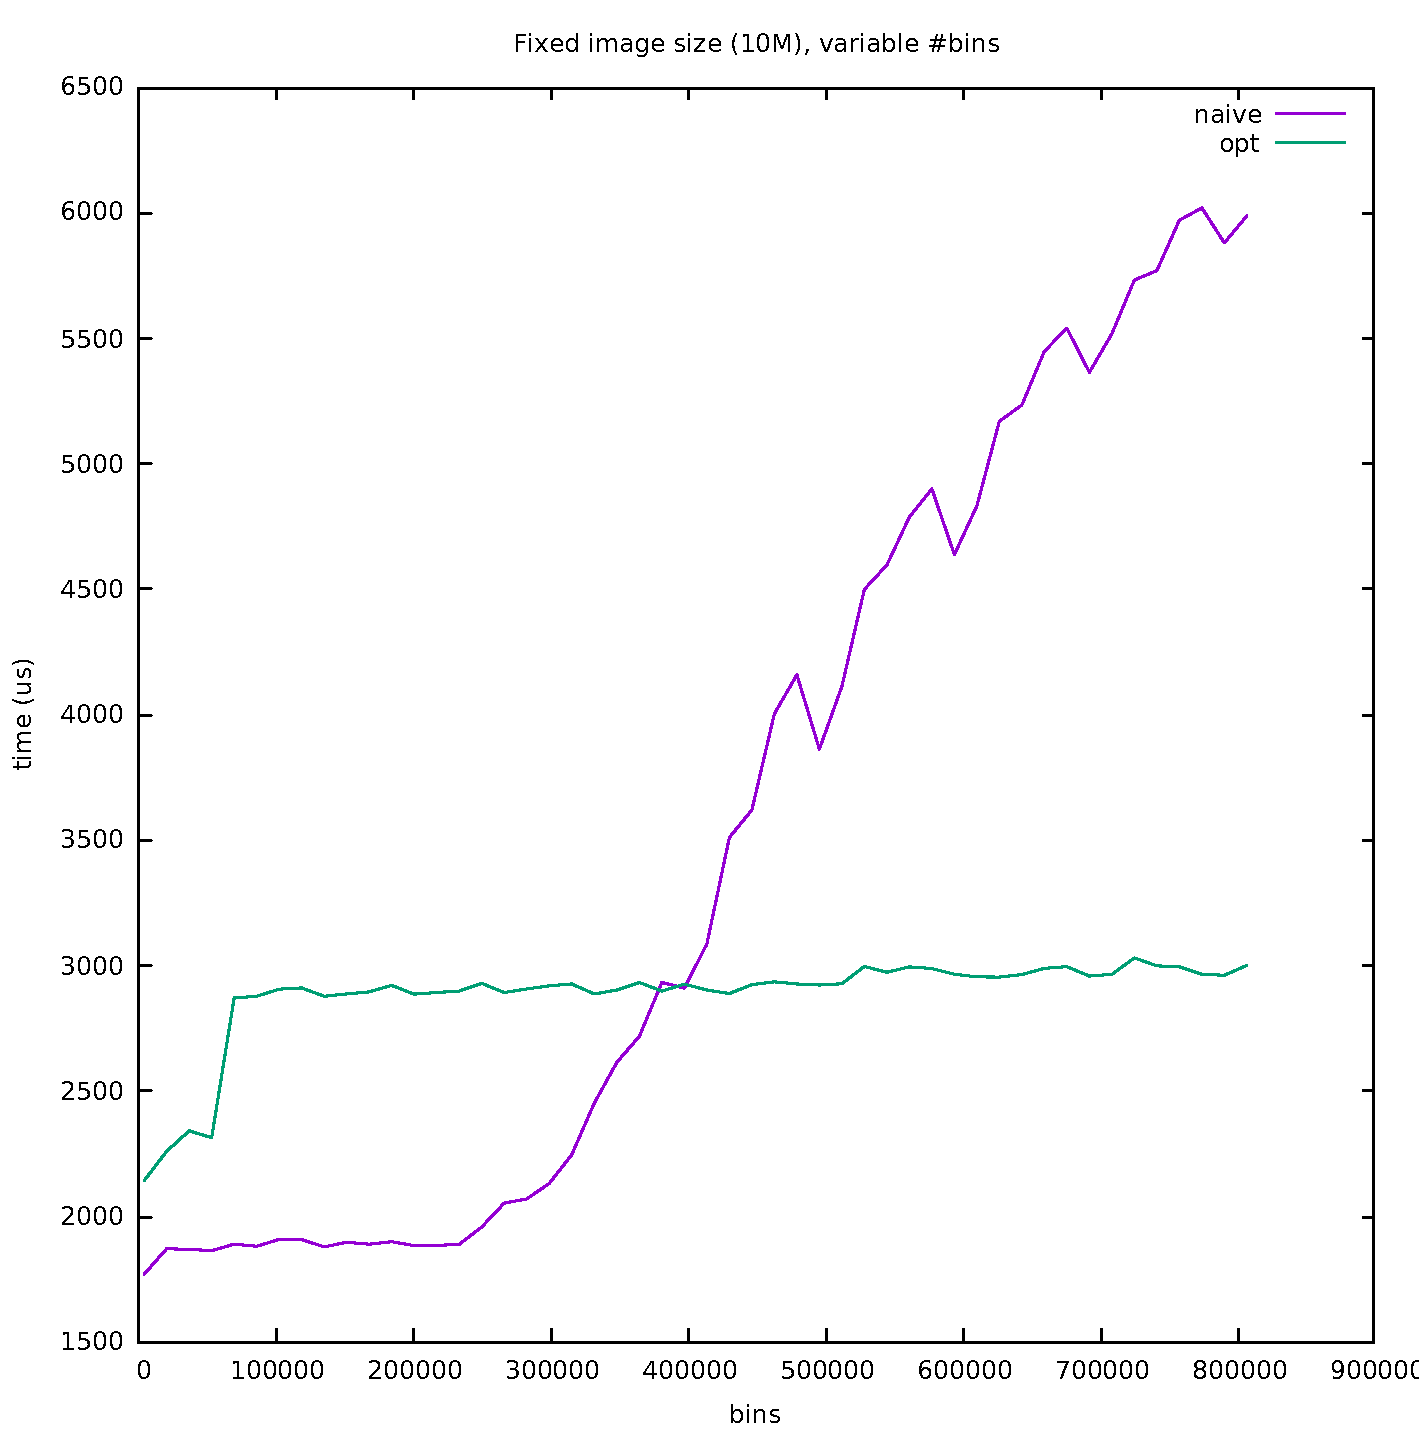
\includegraphics[width=0.6\linewidth]{img/graphs/10M-varbins.pdf}
    \caption{10 million elements with a variable bin count.}
    \label{fig:graph1}
\end{figure}
The benchmark shows that somewhere between 300k and 400k bins,
the optimised implementation is faster.
This seems like a lot of bins,
so we use nvprof to see what kernels dominate the runtime.
The following measurements is for 10M elements and 350k bins.
The result of this is shown in table~\ref{table:nvprof0}.

\begin{table}
    \begin{center}
        \begin{tabular}{l|r|r}
            \bf{Kernel} & \bf{Optimised (us)} & \bf{Naive (us)}   \\ \fatline
            \tt{Index and boundary calculation} & $537$  & $537$  \\ \hline
            \tt{Segment offsets}                & $417$  & -      \\ \hline
            \tt{Radix sort}                     & $1228$ & -      \\ \hline
            \tt{Histogram kernel}               & $446$  & $1433$ \\ \fatline
            \bf{Total}                          & $2628$ & $1970$ \\
        \end{tabular}\\
        \captionof{table}{
          The time spent for various kernels,
          at $10^6$ elements and $3.5 \cdot 10^4$ bins.}
        \label{table:nvprof0}
    \end{center}
\end{table}

It seems like radix sort is very expensive.
It takes almost the same time to do as the naive histogram kernel.
On a more positive note the optimised histogram kernel is about 3 times as
fast as the naive kernel. A possible explanation might be that radix sort
from the Cub library sorts on more bits than we need. We also benchmark
for a smaller dataset (1M). This can be seen on figure~\ref{fig:graph2}.

\begin{figure}[htpb]
    \centering
    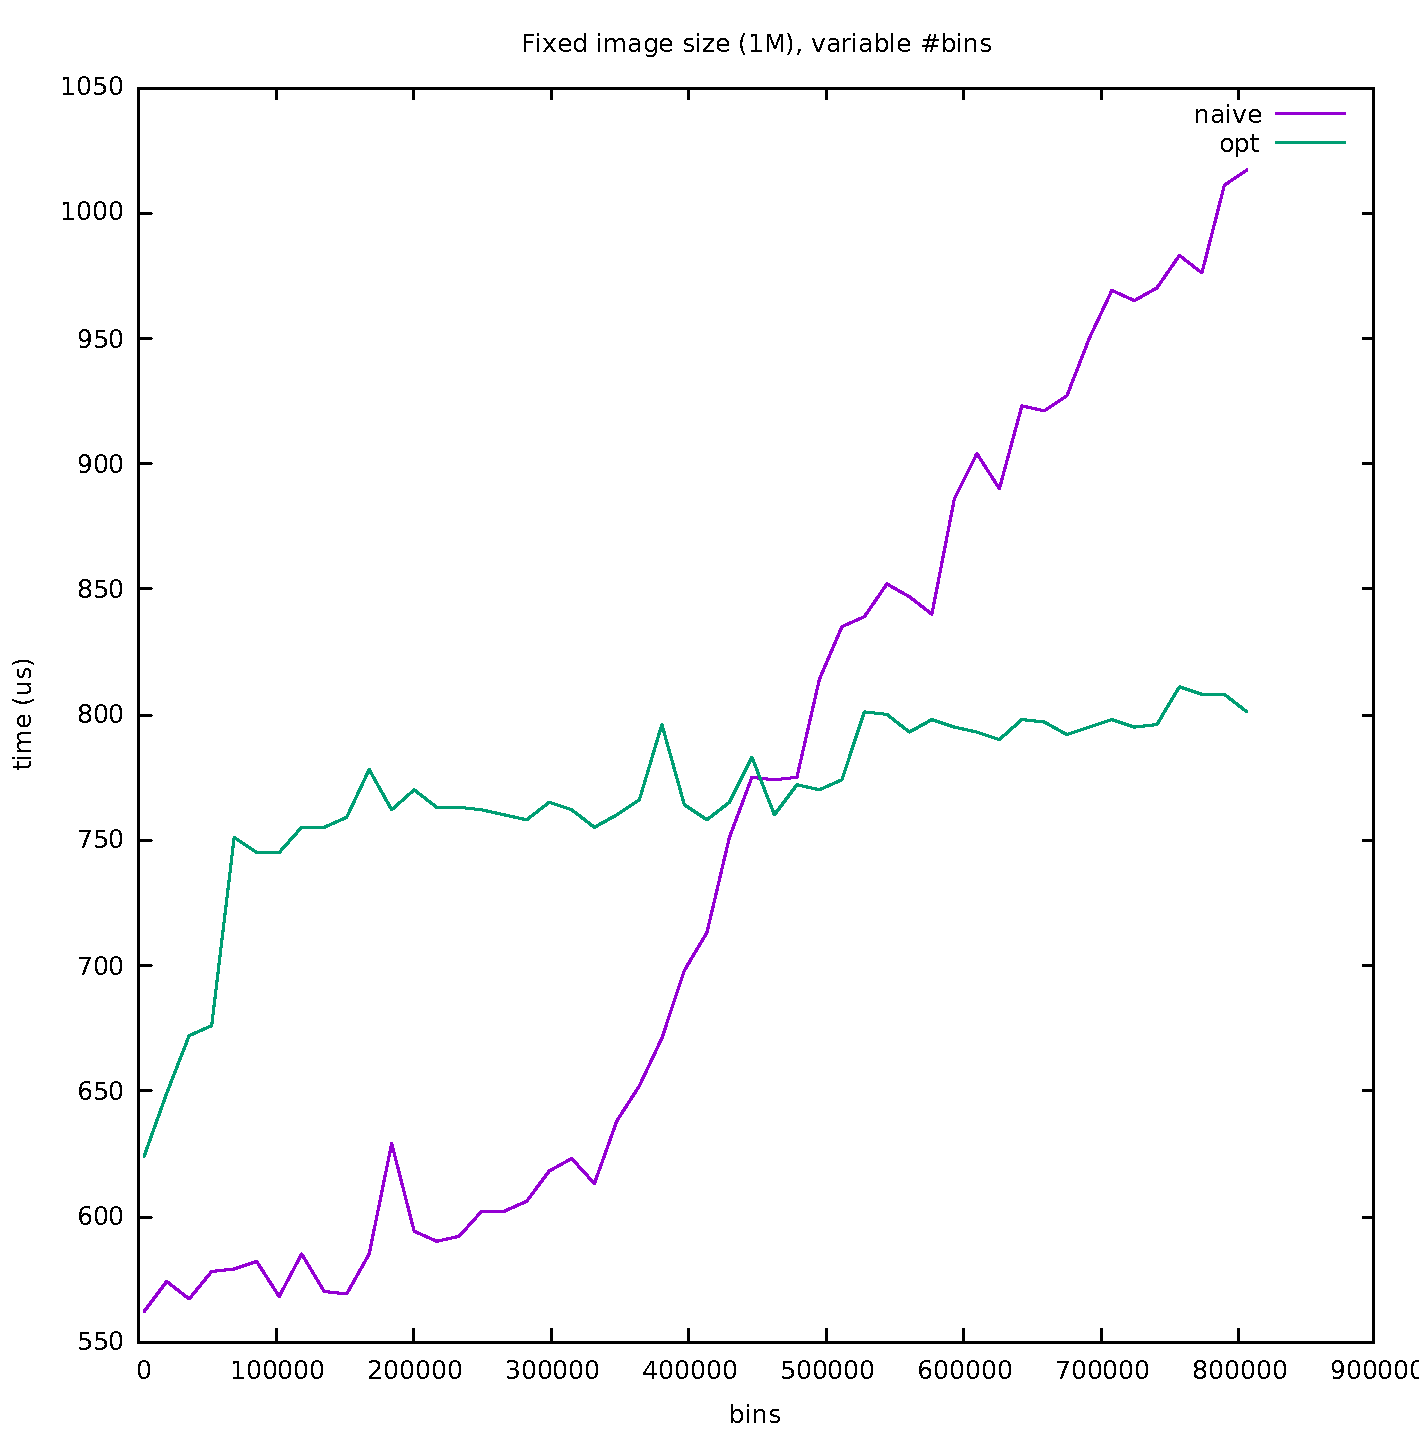
\includegraphics[width=0.6\linewidth]{img/graphs/1M-varbins.pdf}
    \caption{1 million elements with a variable bin count.}
    \label{fig:graph2}
\end{figure}

The results are similar.
We have also benchmarked the kernel optimised for smaller histograms. Again we keep the size of the input array constant, and vary the number of bins. The result can be seen on figure~\ref{fig:graph3} and on figure~\ref{fig:graph4}.

\begin{figure}[htpb]
    \centering
    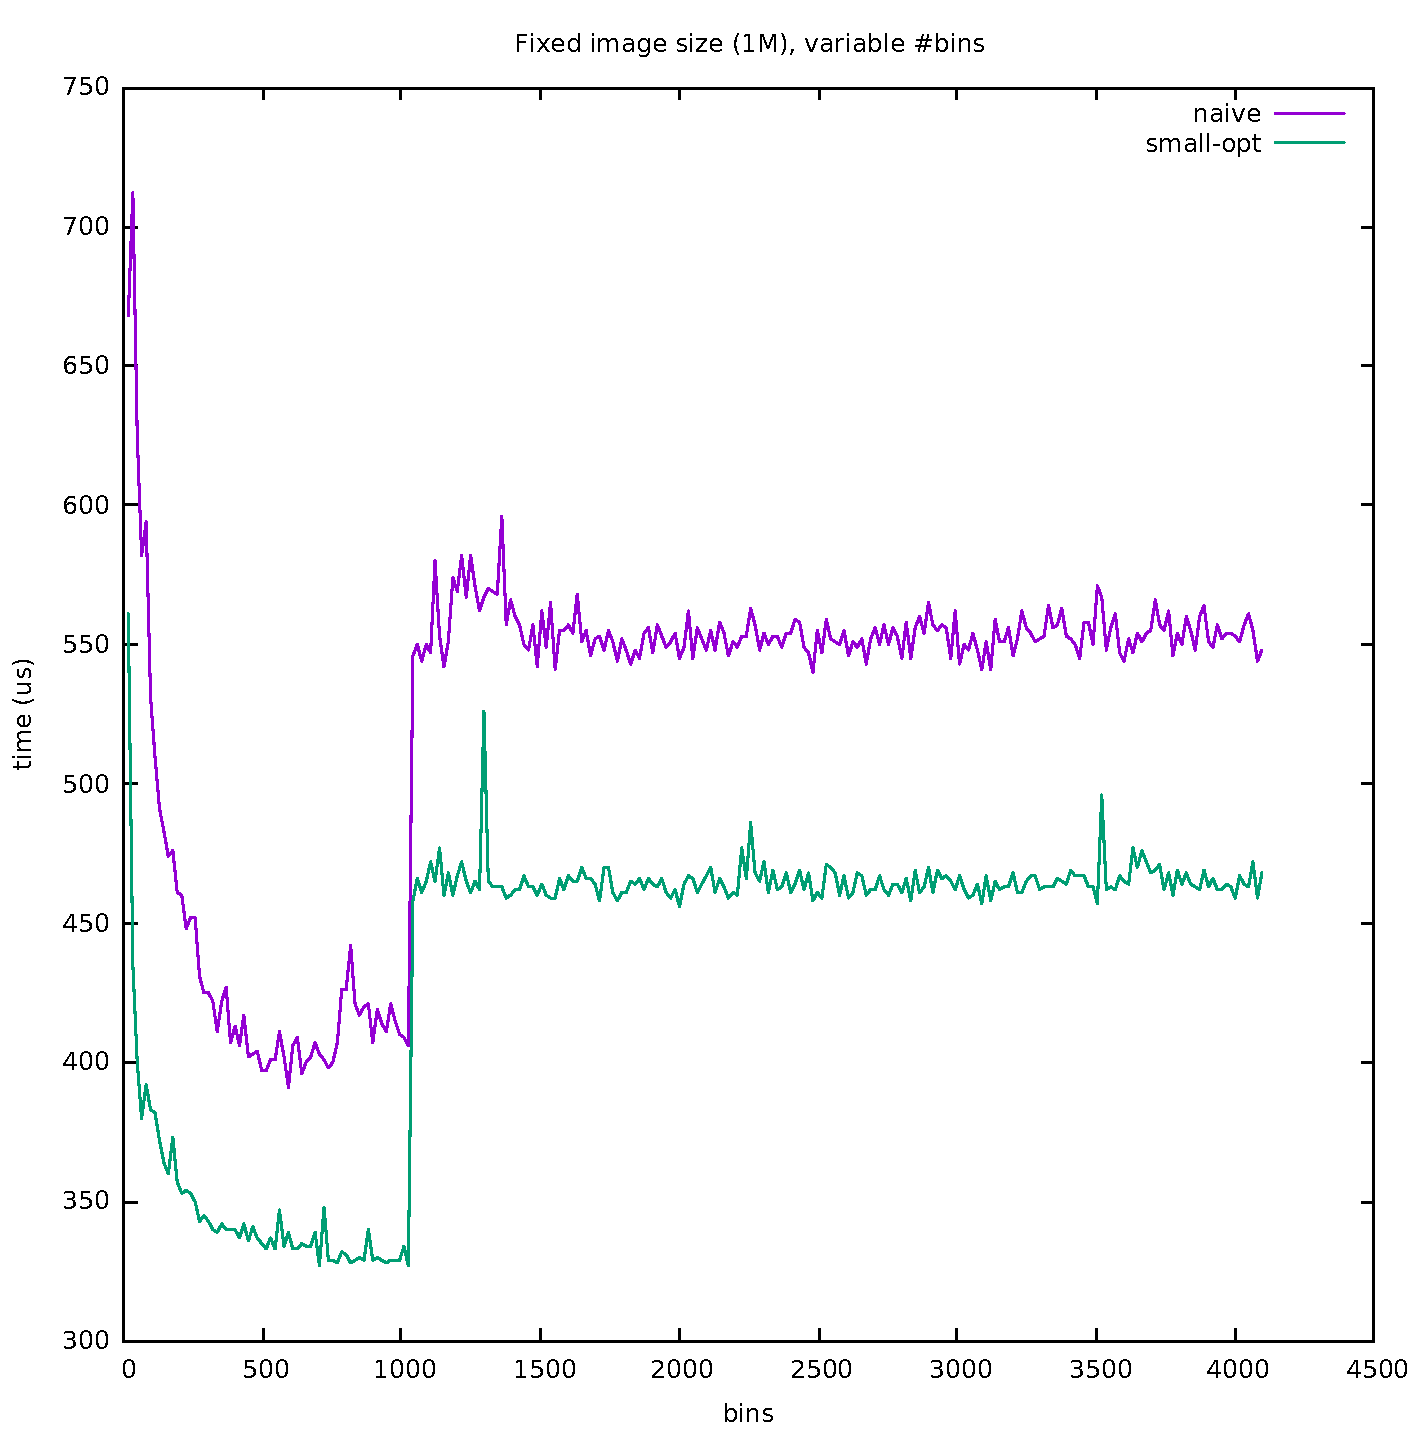
\includegraphics[width=0.6\linewidth]{img/graphs/1M-smallvarbins.pdf}
    \caption{1 million elements with a small variable bin count.}
    \label{fig:graph3}
\end{figure}
\begin{figure}[htpb]
    \centering
    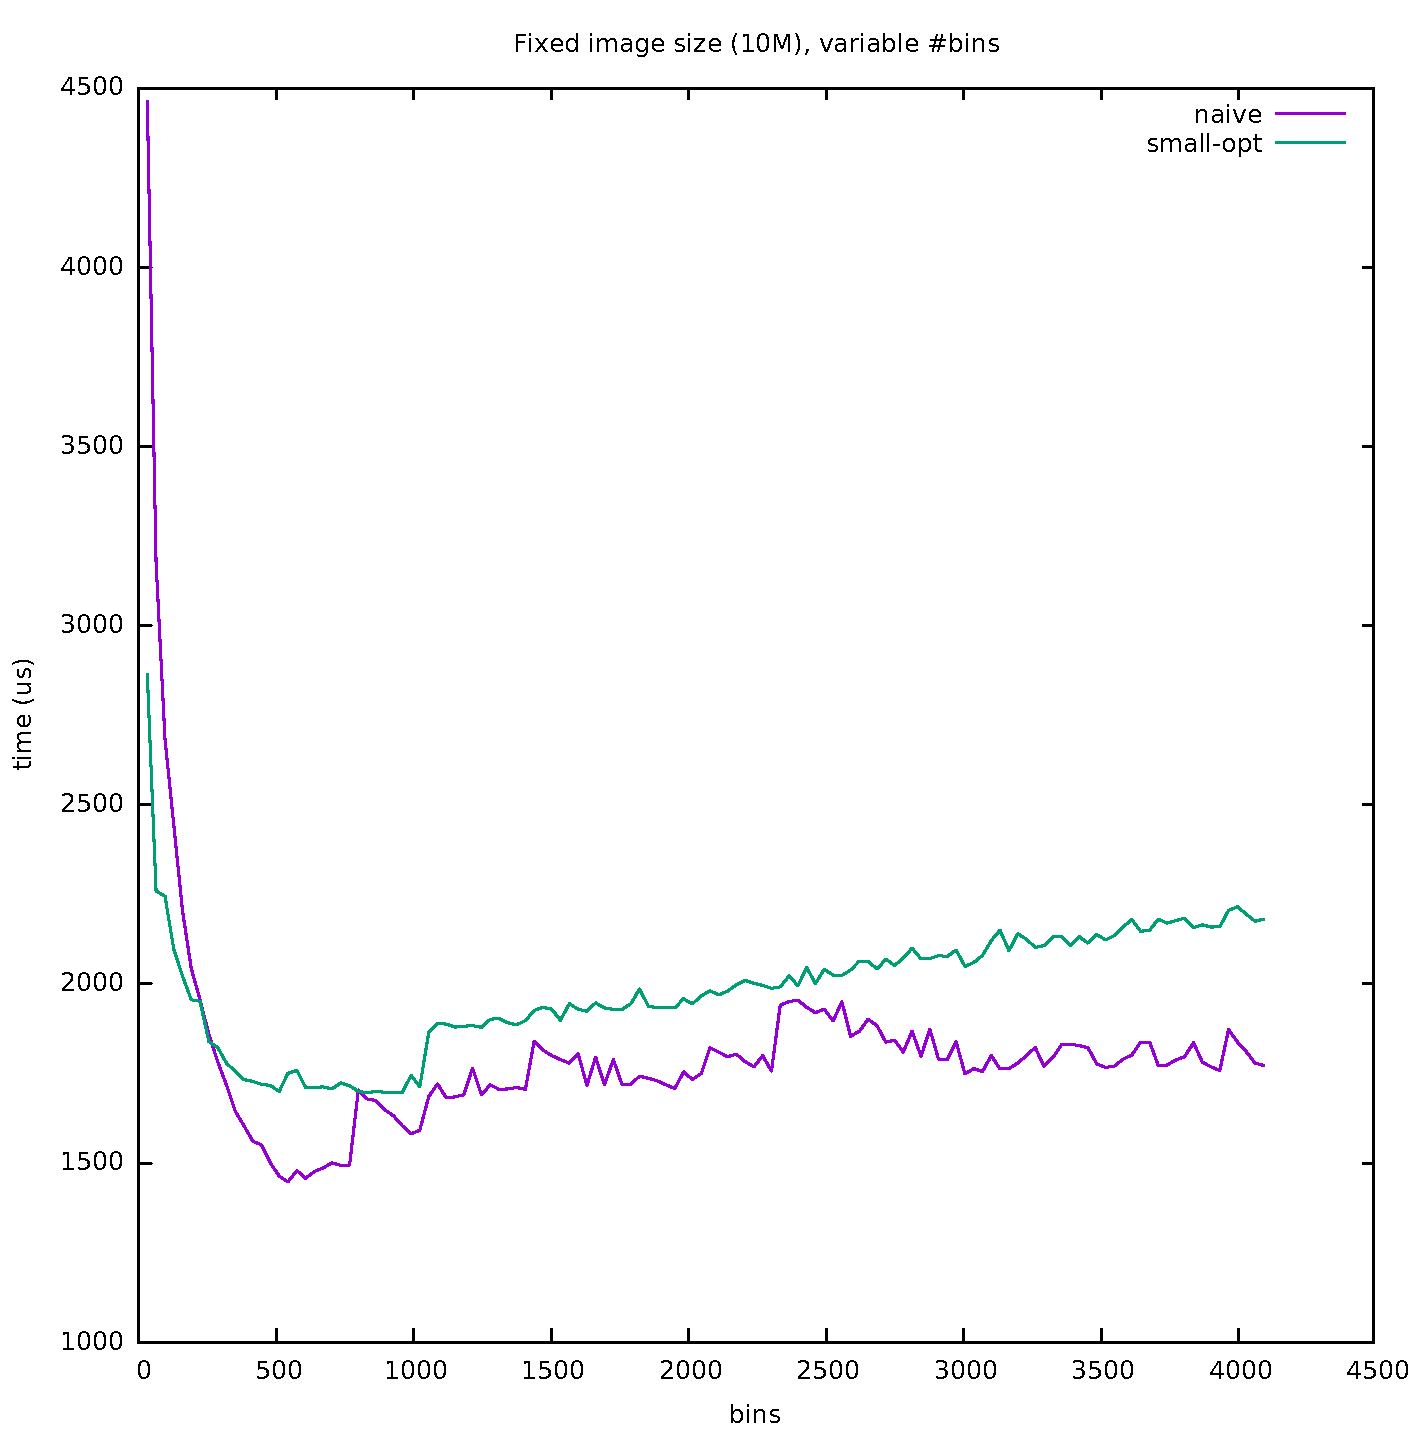
\includegraphics[width=0.6\linewidth]{img/graphs/10M-smallvarbins.pdf}
    \caption{10 million elements with a small variable bin count.}
    \label{fig:graph4}
\end{figure}

The histogram kernel optimised for small histogram sizes is around
20-30\% faster than the very simple naive version. Both implementations see a spike
around 1k bins.
This is probably the sign of some cache effects. They are also very slow for very few bins.
This is because that we have a lot of synchronised writes to the same memory locations.

\subsection{Streaming histogram computation}
For histograms larger than what fits in global memory on the device, we would like to split
the input array into smaller chunks, and work on them in turn. This gives rise to the possibility
of using streaming in order to fully utilize the hardware. In this case we would like to overlap
computation with copying.

CUDA streams gives us the possibility to do this in a fashion shown on figure~\ref{fig:cuda-stream}.
The figure shows copying to the device (HD), histogram computation (K) and copying back the resulting histogram (DH).

\begin{figure}[htpb]
    \centering
    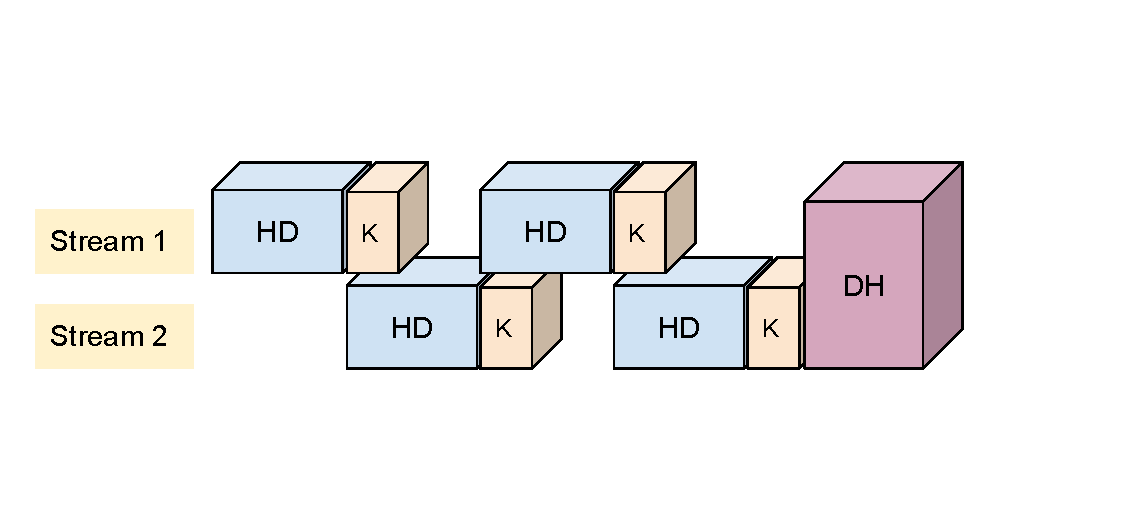
\includegraphics[width=0.8\linewidth]{img/cuda-stream.pdf}
    \captionof{table}{Using streams to overlap copying with computation.}
    \label{fig:cuda-stream}
\end{figure}

For this to work, we need to allocate buffers corresponding to 2 histogram computations.
Then while one buffer is filling up, we are calculating a histogram from the other
buffer. Both are commited to the same histogram.

Because memory copying vastly dominates the runtime of the implementation (90\%),
there is no need to use the optimsed histogram implementation, because the runtime
is limited by the fact that memory transfers are sequential.

We measure this by benchmarking with 1 stream, with 2 streams and on the CPU. 1 stream
is to check whether memory transfers are the dominating factor.

\begin{table}[htpb]
    \centering
    \begin{tabular}{l l}
        Method & Time \\
        \hline
        CPU & 4.6 s \\
        1 stream & 2.5 s \\
        2 streams & 2.5 s \\
        \hline
    \end{tabular}
    \caption{Time of streaming to the device}
    \label{tab:stream}
\end{table}
We test with a data size of 1G elements, and 400k bins. The result is shown in table~\ref{tab:stream}.

This is what we expected, because we deal with a lot of data, and memory transfers to the GPU is
relatively slow compared to computations.

\section{Discussion}
In this section, we give a short dicussion of the genreal problems that we have encountered,
and ..

\subsection{The problem with random access to global memory}
In order to avoid evicting blocks from L1 cache until we are done working with them,
the cuda kernel has to work at small local histograms which fit into shared memory,
then flush back into corresponding parts of the global histogram
in sequential order. Effectively, this means partially sorting the
input data into segments, such that all values in a segment,
contributes to the same small \tt{gpu\_hist\_size} number of bins.
Unfortunately, sorting data and keeping track of segments
introduces great deal of extra work, whose expense has to be compared
with the cost from being very non cache-effective.
A comparison which is done best,
simply by measuring performance on different implementations,
which is exactly what we did.

\subsection{About shared memory.}
Shared memory is divided into equally-sized memory banks.
Any memory read or write request made of $n$ addresses that fall in $n$
distinct memory banks can be serviced simultaneously, yielding an overall bandwidth
that is $n$ times as high as the bandwidth of a single module.
However, if two memory requests fall in the same bank.
The hardware resolves the conflict by serializing the requests,
obviously decreasing throughput by a factor equal to the number of
separate memory requests.

\subsection{Atomic addition}
Imagine a histogram of size 1. Even though the thought is silly,
it reveals a real bottleneck. Since all of the additions to the
histogram must be atomic, the reduction part of the algorithm for
such a small histogram (since all of the additions must be atomic)
exposes exactly 0 parallelism! But as the size of the global histogram
expands, this problem becomes smaller and smaller.
Hence, we expect the parrallel implementation to perform better when the
histogram size expands, for a fixed input data size.

\subsection{Utilizing Available Parallelism}
Theoretically, the amount of time needed to compute a histogram is
proportional with the greatest number of additions to a single bin.
In practice however, this is not the case,
since the available parallelism is limited by physical device resources.
And so the ideal case becomes the one,
where the resources of the hardware is fully utilized at all times.
At a high level of abstraction, this means dividing the workload into
equally sized chunks. The size of a chunk is thus
\tt{total\_workload / hardware\_parallelism}.
Where the total workload in this case is defined as the number of index values
to be computed per thread, and the available parallelism is the number of
threads which can be run at the same time.

\section{Conclusion}
It is in fact possible, to write a computationally efficient and scalable CUDA kernel,
to perform histogram computation for real world unsorted input data.
However

%% NEED TO ANSWER FROM PROBLEM STATEMENT.
%% However, when it comes to real world unsorted data,
%% histograms are computationally inefficient
%% due to the random memory access caused by
%% the counting of how many values fall into each bin.
%% In this project, we implement a CUDA-based solution for building a 1D histogram
%% in parallel and benchmark the scalability of our solution with
%% the CPU and the naive GPU versions.
%% We also investigate how to efficiently solve the problem when the dataset
%% is larger than the available (device) memory on the GPU
%% using streaming techniques.

\section{Further improvements}
Right now we are making a full pass over the index array to calculate
the segment offsets into the index array.
We are pretty sure it would be viable to fuse the segment offset
kernel into the histogram kernel.
Both kernels do a full pass over the index array,
and this would reduce some of the overhead introduced
by the optimised kerned. If successful,
this would reduce reduce the time computing the histogram with a significant factor.


% **************** The End ******************
\end{document}
